\documentclass[paper=a4,UTF8,fontsize=11pt]{scrartcl} % A4 paper and 11pt font size
\usepackage[noend]{algpseudocode}
\usepackage{ctex}
\usepackage[T1]{fontenc} % Use 8-bit encoding that has 256 glyphs
\usepackage{fourier} % Use the Adobe Utopia font for the document - comment this line to return to the LaTeX default
\usepackage[english]{babel} % English language/hyphenation
\usepackage{amsmath,amsfonts,amsthm} % Math packages
\usepackage[english]{babel}
\usepackage[utf8]{inputenc}
\usepackage{indentfirst}
\usepackage{algorithm}
\usepackage{lipsum} % Used for inserting dummy 'Lorem ipsum' text into the template
\usepackage{float}
\usepackage{sectsty} % Allows customizing section commands
\allsectionsfont{\centering \normalfont\scshape} % Make all sections centered, the default font and smaıll caps
\usepackage{graphicx}
\usepackage{fancyhdr} % Custom headers and footers
\pagestyle{fancyplain} % Makes all pages in the document conform to the custom headers and footers
\fancyhead{} % No page header - if you want one, create it in the same way as the footers below
\fancyfoot[L]{} % Empty left footer
\fancyfoot[C]{\thepage} % Empty center footer
\fancyfoot[R]{} % Page numbering for right footer
\renewcommand{\headrulewidth}{0pt} % Remove header underlines
\renewcommand{\footrulewidth}{0pt} % Remove footer underlines
\setlength{\headheight}{13.6pt} % Customize the height of the header
\usepackage[noend]{algpseudocode}
\numberwithin{equation}{section} % Number equations within sections (i.e. 1.1, 1.2, 2.1, 2.2 instead of 1, 2, 3, 4)
\numberwithin{figure}{section} % Number figures within sections (i.e. 1.1, 1.2, 2.1, 2.2 instead of 1, 2, 3, 4)
\numberwithin{table}{section} % Number tables within sections (i.e. 1.1, 1.2, 2.1, 2.2 instead of 1, 2, 3, 4)
\usepackage{color}
\setlength\parindent{0.3pt} % Removes all indentation from paragraphs - comment this line for an assignment with lots of text
\usepackage{graphicx}
\usepackage{xcolor}
\usepackage{listings}
\definecolor{mygreen}{rgb}{0,0.6,0}
\definecolor{mygray}{rgb}{0.5,0.5,0.5}
\definecolor{mymauve}{rgb}{0.58,0,0.82}

\lstset{ 
  language=C++,
  backgroundcolor=\color{white},   % choose the background color
  basicstyle=\footnotesize,        % size of fonts used for the code
  breaklines=true,                 % automatic line breaking only at whitespace
  captionpos=b,                    % sets the caption-position to bottom
  commentstyle=\color{mygreen},    % comment style
  escapeinside={\%*}{*)},          % if you want to add LaTeX within your code
  keywordstyle=\color{blue},       % keyword style
  stringstyle=\color{mymauve},     % string literal style
}
% \lstset{language=C++,
%                 basicstyle=\ttfamily,
%                 keywordstyle=\color{blue}\ttfamily,
%                 stringstyle=\color{red}\ttfamily,
%                 commentstyle=\color{green}\ttfamily,
%                 morecomment=[l][\color{magenta}]{\#}
% }



%----------------------------------------------------------------------------------------
%	TITLE SECTION
%----------------------------------------------------------------------------------------

\newcommand{\horrule}[1]{\rule{\linewidth}{#1}} % Create horizontal rule command with 1 argument of height
\title{
\normalfont \normalsize
\textsc{Shanghai Jiao Tong University} \\ [25pt] % Your university, school and/or department name(s)
\horrule{0.5pt} \\[0.4cm] % Thin top horizontal rule
\huge 最小生成树问题 \\ % The assignment title
\horrule{2pt} \\[0.5cm] % Thick bottom horizontal rule
}

\author{\\ \kaishu 吕艺\\ \normalsize 517021910745} % Your name

\date{\normalsize\today} % Today's date or a custom date

\begin{document}

\maketitle % Print the title
\kaishu
\section{需求分析}

1.本演示文件的主要需求为几个城市之间的通信网络架构问题,主要背景是在n个城市之间以最低的经济代价建设通信网络,是一个最小生成树的问题。
\vspace{0.5cm}

2.演示文件需用户输入,分为用户自行输入数据和自动运行默认数据两种选择。文件运行结束后即在计算机终端上打印路径和最小代价,显示在屏幕上。
\vspace{0.5cm}

3.程序执行的命令包括:

a)用户输入命令(默认参数或手动输入)

b)根据数据建立边表

c)利用Prim算法生成最小生成树

d)将最小生成树以边的文本形式打印在屏幕上,并打印最小代价

\vspace{0.8cm}

\newpage

4.测试数据

顶点集:V=\{a,b,c,d,e,f,g,h\}

边集:E=\{(a,b,4),(a,c,3),(b,c,5),(b,d,5),(b,e,9),(c,d,5)

\qquad \qquad (c,h,5),(d,e,7),(d,f,6),(d,g,5),(d,h,4),(e,f,3),(f,g,2),(g,h,6)\}

\vspace{0.8cm}

\section{概要设计}

本演示文件的主要目标是实现一个最小生成树问题,通过给定的节点以及边的代价,找到遍历节点且代价最低的路径。为了实现这一功能,本演示文件中设计了父类$graph$和派生类$adjListGraph$。

1.父类 $graph$

数据对象: int Ver;\ \ \ \ \ \ \ \ int Edges;

基本操作:virtual bool insert(int s,int e,TypeOfEdge w) = 0;

\qquad \qquad \quad \ \ \ virtual bool remove(int s, int e) = 0;

\qquad \qquad \quad \ \ \     virtual bool exist(int s, int e) const = 0;

\vspace{0.2cm}

2.派生类$adjListGraph$

数据对象: verNode *verList;\ \ \ \ \ \ \ \ int Vers;\ \ \ \ \ \ \ \ int Edges;

私有类:   struct edgeNode \{

    \qquad \qquad \ \  int end;

    \qquad \qquad \ \ TypeOfEdge weight;
    
    \qquad \qquad \ \  edgeNode(int e, TypeOfEdge w, edgeNode *n = NULL)

    \qquad \qquad \ \ { end = e; weight = w; next = n;}
    
    \};
    
    \qquad \qquad \ \ struct verNode \{
        
    \qquad \qquad \ \ TypeOfVer ver; 
    
    \qquad \qquad \ \ edgeNode *head;  
    
    \qquad \qquad \ \ verNode( edgeNode *h = NULL)  { head = h ;}
    
    \};
    
基本操作:adjListGraph(int vSize, const TypeOfVer d[]);

\qquad \qquad \quad \ \ \ 操作条件: 边表还未被初始化

\qquad \qquad \quad \ \ \ 操作结果: 利用传入参数初始化边表

\qquad \qquad \quad \ \ \ bool insert(int u, int v, TypeOfEdge w);

\qquad \qquad \quad \ \ \ 初始条件: 边表已被初始化

\qquad \qquad \quad \ \ \ 操作结果: 插入边

\qquad \qquad \quad \ \ \ bool remove(int u, int v);

\qquad \qquad \quad \ \ \ 初始条件:边表已存在这条边

\qquad \qquad \quad \ \ \ 操作条件: 删除中的指定边

\qquad \qquad \quad \ \ \      bool exist(int u, int v) const;

\qquad \qquad \quad \ \ \  操作条件:边表已被初始化 

\qquad \qquad \quad \ \ \ 操作结果: 寻找边表中是否存在特定边

\qquad \qquad \quad \ \ \ ~adjListGraph() ;

\qquad \qquad \quad \ \ \ 操作条件: 边表已被初始化

\qquad \qquad \quad \ \ \ 操作结果:析构边表,释放内存

\qquad \qquad \quad \ \ \ void prim(TypeOfEdge noEdge) const;

\qquad \qquad \quad \ \ \ 操作条件: 边表已被初始化

\qquad \qquad \quad \ \ \ 操作结果: 输出边和最小代价

\vspace{0.3cm}

2.本程序包括两个模块:

1)  int main() \{
	
	\ \ input order

    \ \  switch(order)\{
			
		\ \ 	 order 1: process default data and print result
		
		\ \  order 2: input data and print result
\}
       
2)  边表单元模块--实现边表的创建以及生成最小生成树

\section{详细设计}
1)边表单元模块
\lstinputlisting{adjgraph.h}

2)主函数模块
\lstinputlisting{main1.cpp}

\vspace{0.3cm}
\section{调试分析}
一开始由于对输入情况考虑的欠缺,本演示文件一开始把边表的节点值设为了字符。为了加强类的泛化能力,本演示文件采用模板类以及模板函数,从而使文件的适用范围更广。

3.算法的复杂度分析

1)时间复杂度
由于采用边表的形式存储,各种操作的算法复杂度比较合理。
$adjListGraph$ 函数的时间复杂度为O(v),主要取决于新建边表时需要赋值的元素个数。
$~adjListGraph$函数的时间复杂度取决于需要释放的元素个数和边条数,故为O(V+E)。
$insert$函数	的时间复杂度为O(1),将插入的节点作为链表的头结点。
$remove$函数	的时间复杂度取决于删除的边在边表中的位置,所以为O(E),
$exist$函数	的时间复杂度取决于指定查找元素在边表中的位置,所以为O(E)
$prim$函数的时间复杂度主要取决于  O(E*V),取决于遍历的次数。
2)空间复杂度

边表模块的空间复杂度与节点的个数与边的条数成正比,即$O(V*E)$。
主函数模块的复杂度取决于定义主函数作用域中的边表,故空间复杂度也为$O(V*E)$。
\vspace{0.5cm}
\section{用户手册}
1.本程序以Jetbrains Clion 2018.2.5, 采用C++ 11 标准,程序以项目方式组织(project),如图1所示:
\begin{figure}[h]
    \centering
    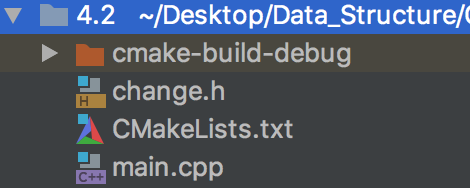
\includegraphics[width=0.8\textwidth]{project.png}
\end{figure}
\vspace{0.2cm}


2.依次点击菜单"Run"->build,再点击"Run",显示文本方式的用户界面,如图 2 所示:
\begin{figure}[h]
    \centering
    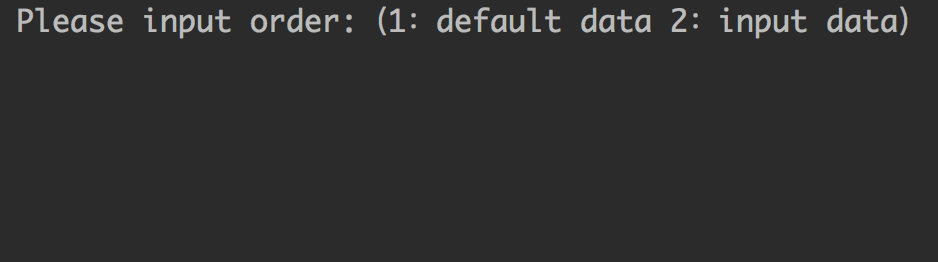
\includegraphics[width=0.8\textwidth]{interface.png}
\end{figure}

\newpage

3.键入操作命令符,1代表使用测试数据,2代表用户自定义参数,之后按“回车键”。程序就执行相应命令。

\section{测试结果}
键入命令1后自动打印默认参数结果

键入命令2后依次输入元素个数,元素值,边(起点 终点 权值),并以空格分开,边输入结束后输入-1以结束输入。
\begin{figure}[h]
    \centering
    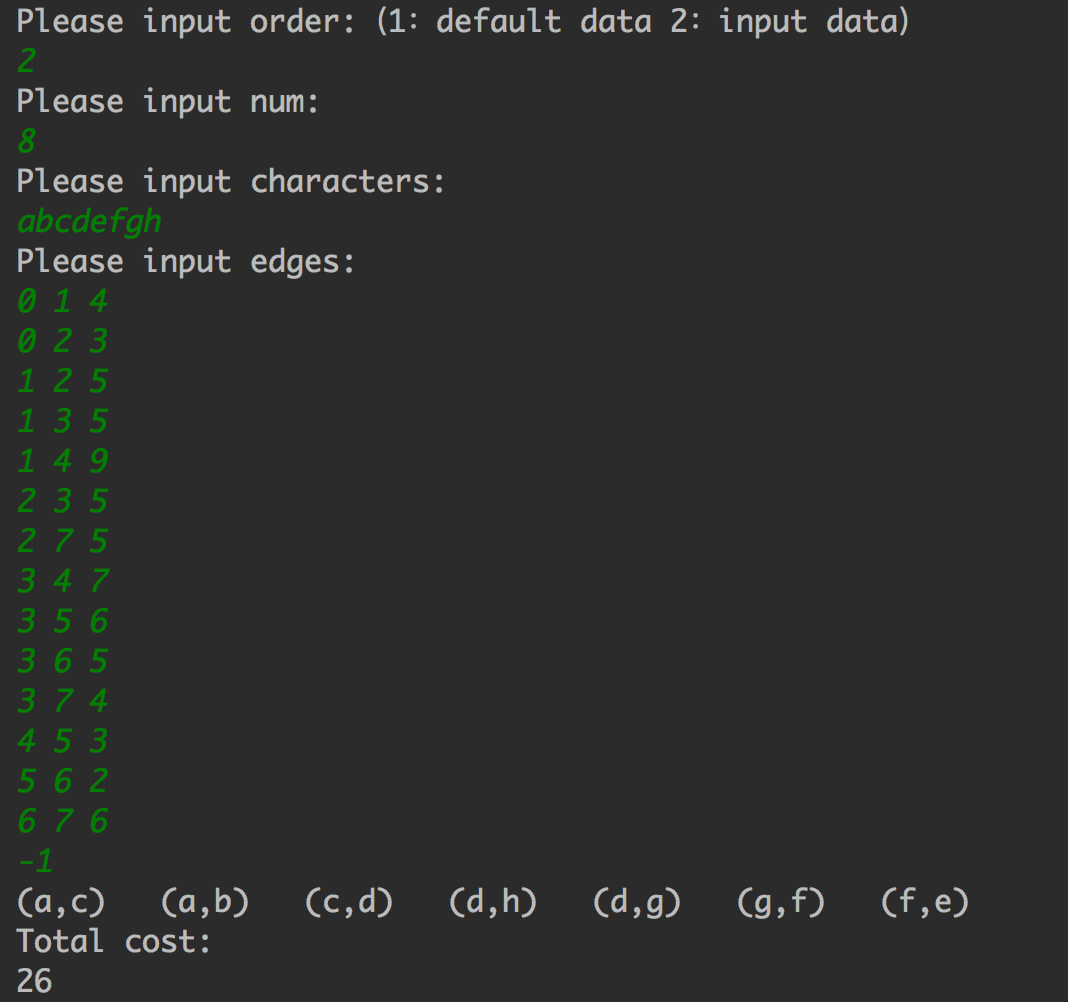
\includegraphics[width=0.4\textwidth]{result.png}
\end{figure}

\section{附录}

源程序文件名清单

main.cpp                //主函数

adjgraph.h              //边表单元模块

\end{document}



